% Copyright 2016 - 2019 Bas van Meerten and Wouter Franssen
%
%This file is part of ssNake.
%
%ssNake is free software: you can redistribute it and/or modify
%it under the terms of the GNU General Public License as published by
%the Free Software Foundation, either version 3 of the License, or
%(at your option) any later version.
%
%ssNake is distributed in the hope that it will be useful,
%but WITHOUT ANY WARRANTY; without even the implied warranty of
%MERCHANTABILITY or FITNESS FOR A PARTICULAR PURPOSE.  See the
%GNU General Public License for more details.
%
%You should have received a copy of the GNU General Public License
%along with ssNake. If not, see <http://www.gnu.org/licenses/>.

\documentclass[11pt,a4paper]{article}
% Copyright 2016 - 2017 Bas van Meerten and Wouter Franssen
%
%This file is part of ssNake.
%
%ssNake is free software: you can redistribute it and/or modify
%it under the terms of the GNU General Public License as published by
%the Free Software Foundation, either version 3 of the License, or
%(at your option) any later version.
%
%ssNake is distributed in the hope that it will be useful,
%but WITHOUT ANY WARRANTY; without even the implied warranty of
%MERCHANTABILITY or FITNESS FOR A PARTICULAR PURPOSE.  See the
%GNU General Public License for more details.
%
%You should have received a copy of the GNU General Public License
%along with ssNake. If not, see <http://www.gnu.org/licenses/>.

\usepackage[british]{babel}
\usepackage{graphicx,booktabs,listings,amsmath,pgfplots,pgfplotstable}
\usepackage[small,bf,nooneline]{caption}
\usepackage{subcaption}
\usepackage[sort&compress,numbers]{natbib}
\usepackage{tikz}
\usepackage{mathtools}
\usepackage[nottoc]{tocbibind}%adds bibliography to table of contents.
\graphicspath{{./images/}}
%\setlength{\textwidth}{453pt} %597 pt is the a4 paperwidth. Minus 2 in margin. 72 pt = 1 in
%\setlength{\hoffset}{-\oddsidemargin}
%\setlength{\voffset}{-30pt} %
%\setlength{\textheight}{651 pt} %a4 height 845 pt minus 2* total headheight. In this case 2*88pt
%% examine margines via the layout package. Use command \layout{} in document to draw a picture.
%\setlength{\parindent}{0.5 cm}
%\setlength{\parskip}{0 cm}
\usepackage[left=82pt,right=82pt,top=95pt,bottom=95pt,footnotesep=0.5cm]{geometry}
%\setlength{\headheight}{14pt}

%define colours--------------------
%dark
\usepackage{xcolor}
\definecolor{MyGrayD}{RGB}{1,1,1}
\definecolor{MyRedD}{RGB}{237,45,46}
\definecolor{MyGreenD}{RGB}{0,140,71}
\definecolor{MyBlueD}{RGB}{24,89,169}
\definecolor{MyOrangeD}{RGB}{243,125,34}
\definecolor{MyPurpleD}{RGB}{102,44,145}
\definecolor{MyBrownD}{RGB}{161,29,32}
\definecolor{MyPinkD}{RGB}{179,56,147}
%normal
\definecolor{MyGray}{RGB}{114,114,114}
\definecolor{MyRed}{RGB}{241,89,95}
\definecolor{MyGreen}{RGB}{121,195,106}
\definecolor{MyBlue}{RGB}{89,154,211}
\definecolor{MyOrange}{RGB}{249,166,90}
\definecolor{MyPurple}{RGB}{158,102,171}
\definecolor{MyBrown}{RGB}{205,112,88}
\definecolor{MyPink}{RGB}{215,127,179}
%light
\definecolor{MyGrayL}{RGB}{204,204,204}
\definecolor{MyRedL}{RGB}{242,174,172}
\definecolor{MyGreenL}{RGB}{216,228,170}
\definecolor{MyBlueL}{RGB}{184,210,235}
\definecolor{MyOrangeL}{RGB}{242,209,176}
\definecolor{MyPurpleL}{RGB}{212,178,211}
\definecolor{MyBrownL}{RGB}{221,184,169}
\definecolor{MyPinkL}{RGB}{235,191,217}
%----------------------------------

%Figure ref with hyperref
\newcommand{\fref}[1]{\hyperref[#1]{Figure \ref*{#1}}}
\newcommand{\sref}[1]{\hyperref[#1]{Section \ref*{#1}}}
\newcommand{\tref}[1]{\hyperref[#1]{Table \ref*{#1}}}

%Makes a new command for figures with input values: filename, width(times linewidth),
% caption and label.
\newcommand{\onefigure}[4]{
\setlength{\captionwidth}{#2\linewidth}
\begin{figure}
\includegraphics[width=#2\linewidth]{#1}
\centering
\parbox{\linewidth}{\caption{#3}
\label{#4}}
\end{figure}
}

%Makes a new command for tikz figures with input values: tikz commands, 
% caption and label.
\newcommand{\onetikz}[3]{
\settowidth{\captionwidth}{#1}
\ifthenelse{\lengthtest{\captionwidth<0.7\linewidth}}{\setlength{\captionwidth}{0.7\linewidth}}{}

\begin{figure}
\centering
#1
\centering
\parbox{\linewidth}{\caption{#2}
\label{#3}}
\end{figure}
}

%Makes a new command for two figures next to each other with input values: filename1, caption1, label1,filename2, caption2 and label2. Figure width is set to 0.47\linewidth and the space between the figures is filled with \hfill so the sides of the figures align with to edge of the line.
\newcommand{\twofigure}[6]{
\setlength{\captionwidth}{\linewidth}
\begin{figure*}[ht!]
\begin{minipage}[t]{0.47\linewidth}
\includegraphics[width=\linewidth]{#1}
\centering
\caption{#2}
\label{#3}
\end{minipage}
\hfill
\begin{minipage}[t]{0.47\linewidth}
\centering
\includegraphics[width= \linewidth]{#4}
\centering
\caption{#5}
\label{#6}
\end{minipage}
\end{figure*}
}


%Makes a new command for a table with caption witdh equal to the total table width. Input: tabular, caption and label. Example:
%\onetable{
%\begin{tabular}{ccc}
%a&b&c\\
%\hline
%1&1&1\\
%1&1&1\\
%1&1&1\\
%\end{tabular}
%{The caption.}
%{tab:table1}
%}
\newcommand{\onetable}[3]{
\settowidth{\captionwidth}{#1}
\ifthenelse{\lengthtest{\captionwidth<0.7\linewidth}}{\setlength{\captionwidth}{0.7\linewidth}}{}
\begin{table}
\caption{#2}
\vspace{-0.24cm} %Puts caption close to toprule
\label{#3}
\centering
#1
\end{table}
}

%Makes a long table with captionwidth equal to tablewidth. It takes the following arguments:
%1: Column specifier (e.g. cccc)
%2: Caption
%3: Label
%4: First head (i.e. first row of regular table)
%5: Head of consecutive pages
%6: Foot of pagebreak
%7: Lastfoot (e.g. \midrule)
%8: Body of table
\newcommand{\onelongtable}[8]{
\begin{center}
\settowidth{\captionwidth}{
\begin{tabular}{#1}
#4
#8
\end{tabular}} % This ends the captionwidth part. Next comes the real table.

\begin{longtable}{#1}
\caption{#2}\\
\vspace{-0.74cm} %Puts caption close to toprule
\label{#3}\\

#4
\endfirsthead

#5
\endhead

#6
\endfoot

#7
\endlastfoot

#8
\end{longtable}
\end{center}}




%1:pgfplots code
%2:width
%3:caption
%4:label
\newcommand{\pgfplotsfigure}[4]{
\pgfplotsset{width=#2\linewidth}
\setlength{\captionwidth}{#2\linewidth}
\begin{figure}[t]
\centering
#1
\centering
\parbox{\linewidth}{\caption{#3}
\label{#4}}
\end{figure}
}


\usepackage[bitstream-charter]{mathdesign}
\usepackage[T1]{fontenc}
\usepackage[protrusion=true,expansion,tracking=true]{microtype}
\pgfplotsset{compat=1.7,/pgf/number format/1000 sep={}, axis lines*=left,axis line style={gray},every outer x axis line/.append style={-stealth'},every outer y axis line/.append style={-stealth'},tick label style={font=\small},label style={font=\small},legend style={font=\footnotesize}}
\usepackage{colortbl}
\usetikzlibrary{calc}

%Set section font
\usepackage{sectsty}
\allsectionsfont{\color{black!70}\fontfamily{SourceSansPro-LF}\selectfont}
%--------------------


%Set toc fonts
\usepackage{tocloft}
%\renewcommand\cftchapfont{\fontfamily{SourceSansPro-LF}\bfseries}
\renewcommand\cfttoctitlefont{\color{black!70}\Huge\fontfamily{SourceSansPro-LF}\bfseries}
\renewcommand\cftsecfont{\fontfamily{SourceSansPro-LF}\selectfont}
%\renewcommand\cftchappagefont{\fontfamily{SourceSansPro-LF}\bfseries}
\renewcommand\cftsecpagefont{\fontfamily{SourceSansPro-LF}\selectfont}
\renewcommand\cftsubsecfont{\fontfamily{SourceSansPro-LF}\selectfont}
\renewcommand\cftsubsecpagefont{\fontfamily{SourceSansPro-LF}\selectfont}
%--------------------


\usepackage[hidelinks,colorlinks,allcolors=black, pdftitle={Diffusion analysis in ssNake},pdfauthor={Wouter M.J.\ Franssen}]{hyperref}

\interfootnotelinepenalty=10000 %prevents splitting of footnote over multiple pages
\linespread{1.2}

\title{\color{black}\fontfamily{SourceSansPro-LF}\bfseries Diffusion analysis in ssNake}
\author{}
\date{\color{black}\fontfamily{SourceSansPro-LF}\bfseries \today}


\begin{document}
%\newgeometry{left=72pt,right=72pt,top=95pt,bottom=95pt,footnotesep=0.5cm}
\microtypesetup{protrusion=true} % enables protrusion

\maketitle

\section{Introduction}
Is this tutorial, we will analyse a diffusion measurement of a liquid state sample in ssNake.
Diffusion is a powerful tool to distinguish multiple molecules in complicated spectra, especially when
other 2D methods cannot readily identify the different components. The diffusion experiment consists
of a spin-echo experiment, with gradients present during the echo time. In case of no diffusion,
each nucleus experiences the same B$_0$ field during the first part of the echo as during the last,
and perfect echo refocussing occurs. In case of displacements in this time (i.e.\ diffusion), the
B$_0$ field are different during part 1 and part 2 of the echo, and attenuation of the signal occurs.
If the strength and durations of the gradients are known, the diffusion constant can be extracted
from such a measurement.


\section{Data}
The data for this tutorial was recorded at 300 MHz.
The sample was a tube of pure water.
The maximum gradient strength was 1.5 T/m. The relevant times were: $\delta = 1$ ms, and $\Delta = 20$ ms.

\section{Fitting a diffusion curve}
Start by loading the Bruker type data:
\begin{itemize}
  \item Load the `ser' file that was delivered with this tutorial
\end{itemize}

Now, we want to zero-fill the data, as well as correct for the Bruker time delay (i.e.\ digital
filter). It is best to do the zero-filling first:
\begin{itemize}
  \item Use `Matrix $\longrightarrow$ Sizing', and set the size to 65536
  \item Correct the digital filter by using `Tools $\longrightarrow$ Correct digital filter'
  \item Fourier transform
\end{itemize}
Correct for the phasing:
\begin{itemize}
  \item Phase using `Tools $\longrightarrow$ Phasing' with -118.470 zero order.
\end{itemize}
Now, we will analyse the intensity variation of this peak. In
order to do this, we will integrate this region.
\begin{itemize}
  \item Use `Matrix $\longrightarrow$ Region $\longrightarrow$', and integrate between point 31393
	 and 33638. (Or left click on the left and right side of the relevant peak in the spectrum.)
\end{itemize}
This should show:
\begin{center}
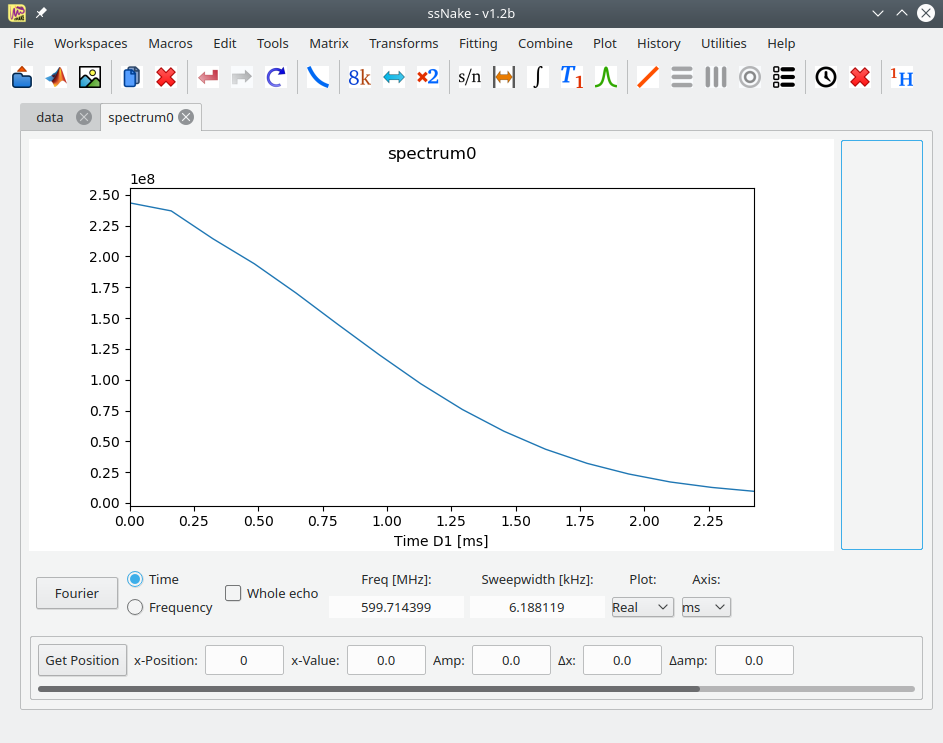
\includegraphics[width=0.8\linewidth]{Figs/Fig1.png}
\end{center}
which shows  a nice Gaussian decay due to the diffusion.

Now, we want to fit this decay, which means that we must supply ssNake with the relevant x-axis. In
this case, we have measured multiple spectra with a different gradient strengths. The strengths were
approximately linear, with real values: 4.995005e-03, 7.132867e-02, 1.376623e-01,
2.039960e-01, 2.703297e-01, 3.366633e-01, 4.029970e-01,
4.693307e-01, 5.356643e-01, 6.019980e-01, 6.683317e-01,
7.346653e-01, 8.009990e-01, 8.673327e-01, 9.336663e-01,
1.000000e+00.

These are the values passed to the pulse sequence. 1 stands for the maximum gradient strength of the machine. In this case this is 1.5 T/m. Additionally, the puls esequence itself caps the gradient at 90\% for safety reasons.

With these values, we must change the
x-axis in ssNake:

\begin{itemize}
  \item Use `Plot $\longrightarrow$ User x-axis' and fill in: array([4.995005e-03, 7.132867e-02, 1.376623e-01,
2.039960e-01, 2.703297e-01, 3.366633e-01, 4.029970e-01,
4.693307e-01, 5.356643e-01, 6.019980e-01, 6.683317e-01,
7.346653e-01, 8.009990e-01, 8.673327e-01, 9.336663e-01,
1.000000e+00])*1.5*0.9
\item Set the Axis unit to `s'
\end{itemize}
Here, we make use of ssNake's calculation capability to multiply the array by some values. Note that
the axis still shows `Time D1 [s]', while actually it is a gradient strength T/m (you need to remember
this for yourself!).

The final step is to fit this curve using the Diffusion fit method of ssNake.

\begin{itemize}
  \item Use `Fitting $\longrightarrow$ Diffusion Curve'.
  \item Set $\delta$ to 1e-3.
  \item Set $\Delta$ to 20e-3.
  \item Fix the Coefficient by ticking the box next to it.
  \item Push `Fit'. (Might need a second push to do a second fit run.)
\end{itemize}
This should lead to a D value of 1.938e-09 m$^2$/s, which is a typical value for pure water at room temperature.

The fit looks like:
\begin{center}
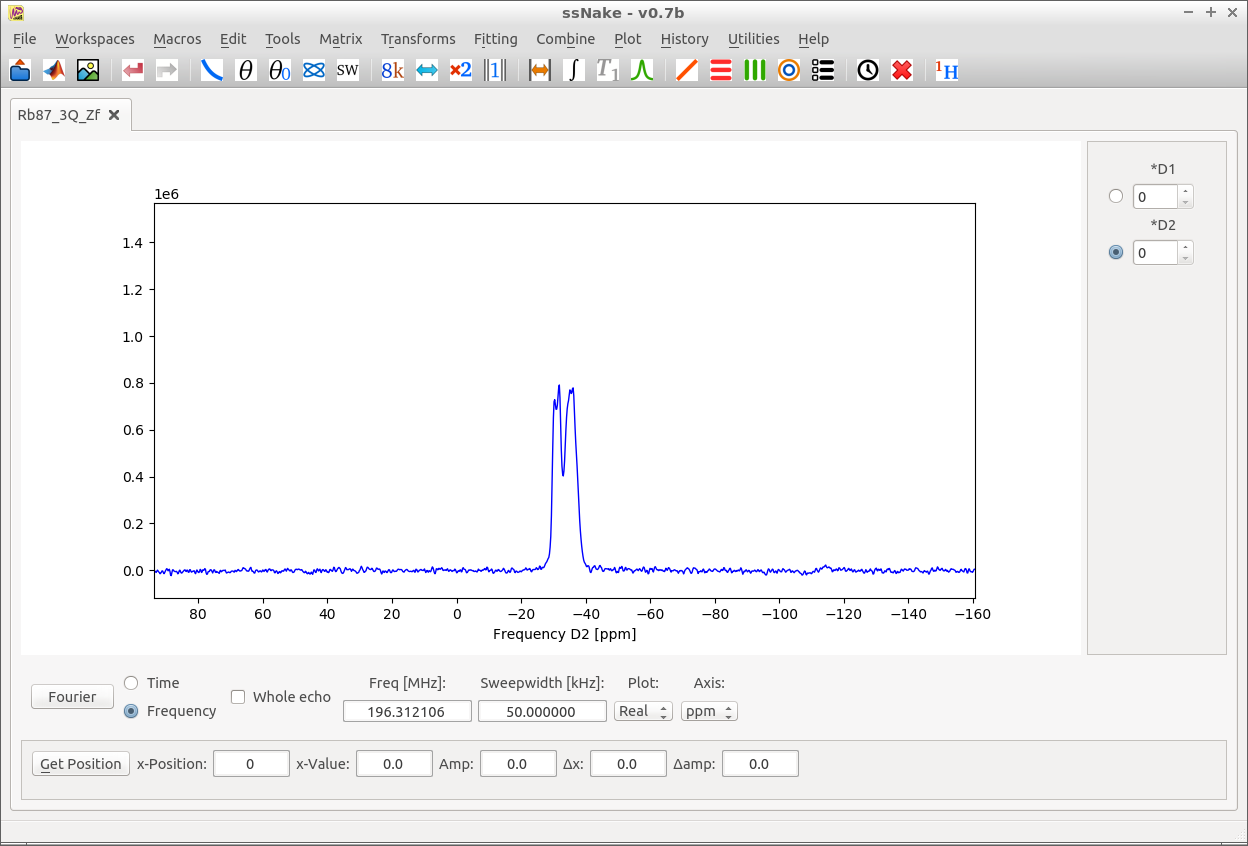
\includegraphics[width=0.8\linewidth]{Figs/Fig2.png}
\end{center}
which is an excellent fit.

\section{Pitfalls}
It can sometime be difficult to establish the true gradients used by the spectrometer. At least in my experience, Bruker Topspin handles this a bit weirdly. While other parameters (pulse lengths, delays etc.) are saved in the parameter files, the gradient list is in an external file. As shown above, some recalculation is needed to get the gradient values in T/m from these. When setting op these measurements, it might be wise to do a check on a sample of pure water, to verify if your methods are correct.

The diffusion equation used in ssNake is applicable for the most common diffusion sequences (spin echo and stimulated echo). When using a stimulated echo with bi-polar gradients, note that the length $\delta$ signifies the total time of both gradient lobes combined.

When the gradient pulses are not rectangular (e.g.\ trapezoidal), the time $\delta$ needs to be corrected for this before fitting.

\end{document}
